\section{Wednesday}\index{Wednesday_lecture}
\subsection{Epidemiology}
Population $N$ fixed (ignoring birth, death, $\dots$)\\
S(t): the number of individuals in the susceptible class.\\
I(t): the number of individuals in the infected class.\\
R(t): the number of individuals in the removed class.\\
Rate of change of $S(t)$ is proportional to the product of $S(t)\&I(t)$.\\
Rate of change of $R(t)$ is proportional to hte size of $I(t)$.\\
\[\begin{cases}\dot{s}=-rsI\\\dot{I}=rsI-\delta I\\\dot{R}=\delta I\end{cases}
\]
\[\frac{dI}{ds}=\frac{\dot{I}}{\dot{s}}=\frac{rsI-\delta I}{-rsI}=-1+\frac{\delta}{r}\frac{1}{S}\]
\[I(t)-I(0)=-(s-s_0)+\frac{\delta}{r}ln\frac{s(t)}{s_0}
\]
\[I(t)=I_0+s_0-s+\rho ln\frac{s}{s_0},\qquad \rho=\frac{\delta}{r}
\]
as $s\rightarrow0, I\rightarrow-\infty ~0=-1+\rho\frac{1}{s},~s=\rho$
\begin{figure}[H]
\centering
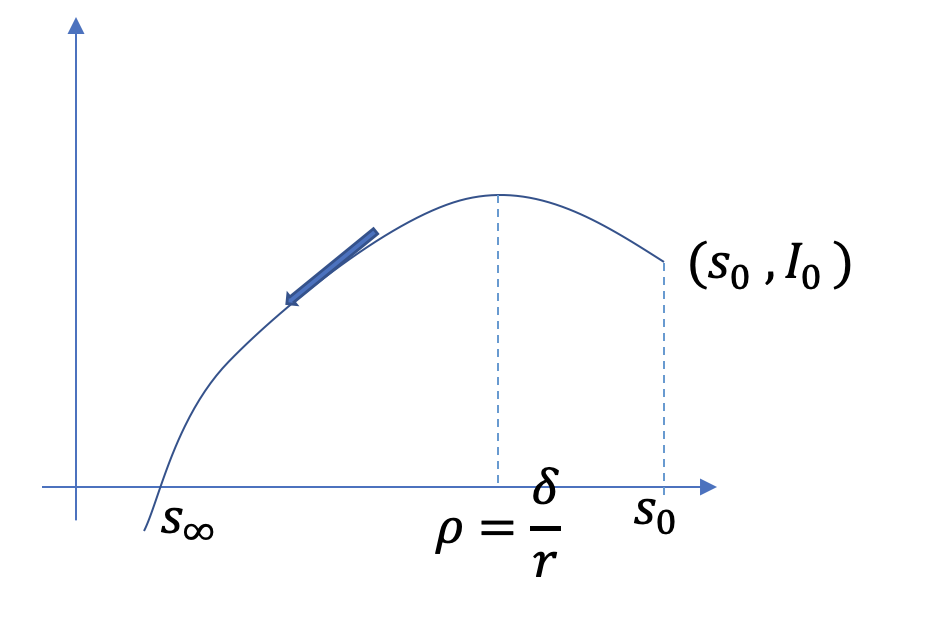
\includegraphics[width=8cm]{week14}
\end{figure}









